\bodychapter{INTRODUCTION: A REALLY LONG CHAPTER TITLE THAT SPANS MULTIPLE LINES SHOULD BE SINGLE-SPACED IN THE TEXT}
\label{Intro}

There is a substantial body of work in HCI that guides the evaluation of productivity support tools. Shneiderman compared the growing community of researchers developing and studying creativity support tools to the earlier rise of researchers working on productivity support tools~\cite{Shneiderman:2007wp}. He said that researchers in CSTs are ``moving from the comparatively safe territory of productivity support tools to the more risky frontier of creativity support tools.'' Shneiderman noted that one of the challenges that makes CST research `risky' is that there are no obvious measures of success~\cite{Shneiderman:2007wp}. 

\begin{table}[t]
\centering
\scriptsize
\caption[Overview of Creativity Support Tools]{A summary of creativity support tools, including examples from research and industry.}
\begin{tabular}{|l|l|}
\hline
\textbf{Category} & \textbf{Example} \\
\hline
Visualization \& Simulation  & Tableau, D3, netLogo \\
Concept Mapping \& Information Collage & combinFormation, Visio, Omnigraffle \\
Architectural \& Design & AutoCAD, Rhino3D \\ 
Mathematics & SPSS, MatLab, WolframAlpha \\
Software development environments & Eclipse, Visual Studio \\
Video Editing & Final Cut Pro, iMovie \\
Drawing/Painting &  Illustrator, InkScape, CorelDraw \\
Animation & Flash, Maya, SoftImage, Houdini \\
Music & GarageBand, Zya, Sequel, NodeBeat \\
Photography & Photoshop, Lightroom \\
Wikis, Blogs, \& Online Presence  & MediaWiki, WordPress, DreamWeaver \\
Writing \& Presentation & Google Docs, MS Word, Prezi \\
\hline
\end{tabular}
\label{CSTSummary}
\end{table}%

\begin{figure}[t]
\centering
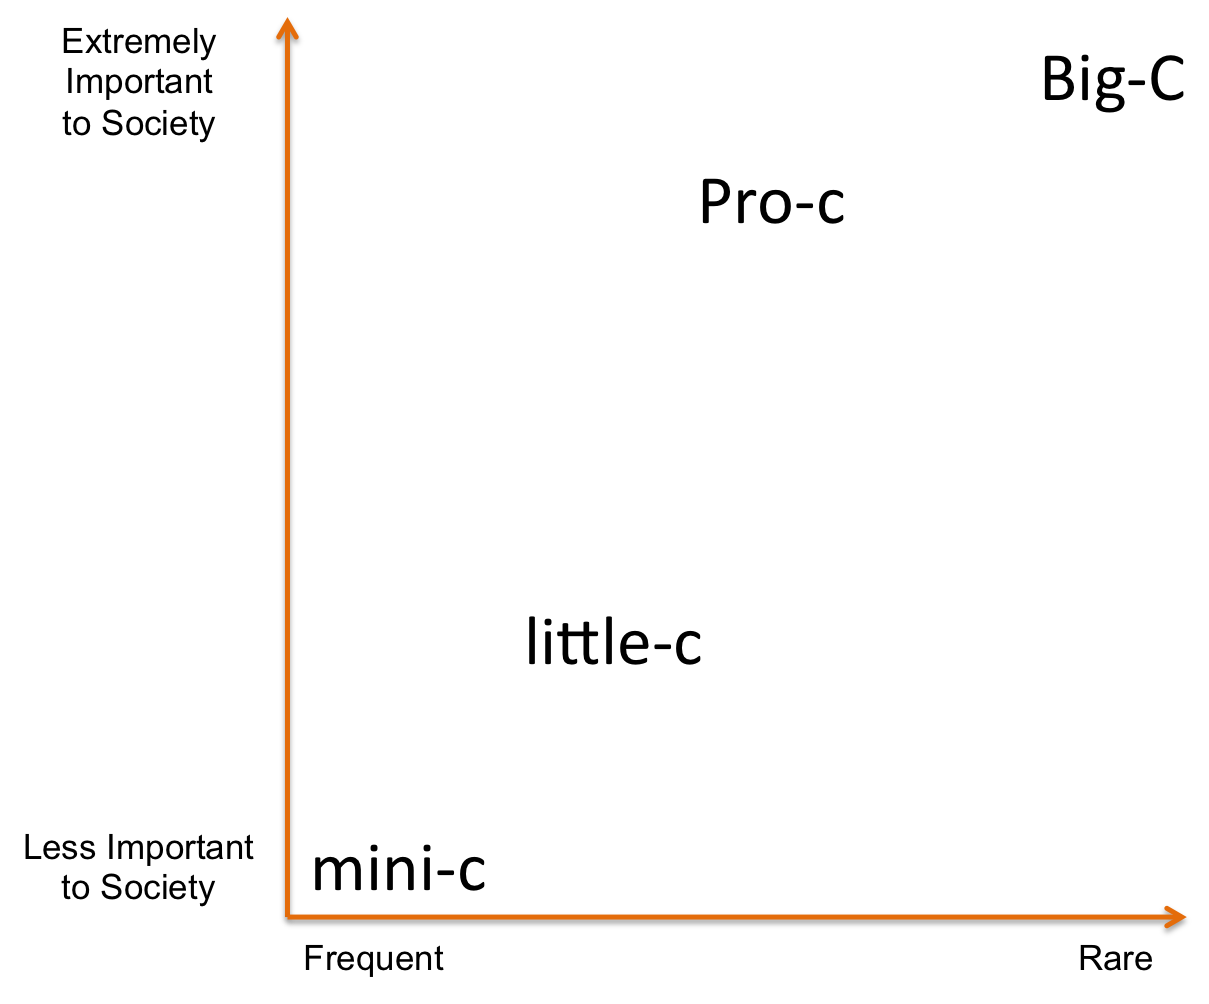
\includegraphics[width=4in]{images/spectrum.png}
\caption[Novelty-Impact Space of Creativity (Along with some extra text that makes multiple lines)]{The creativity literature contains classifications of creative contributions across two dimensions: the Novelty-Impact space. Highly novel contributions are more rare, contributions with minimal novelty are more frequent.}
\label{NIspace}
\end{figure}

\begin{figure}[t]
\centering
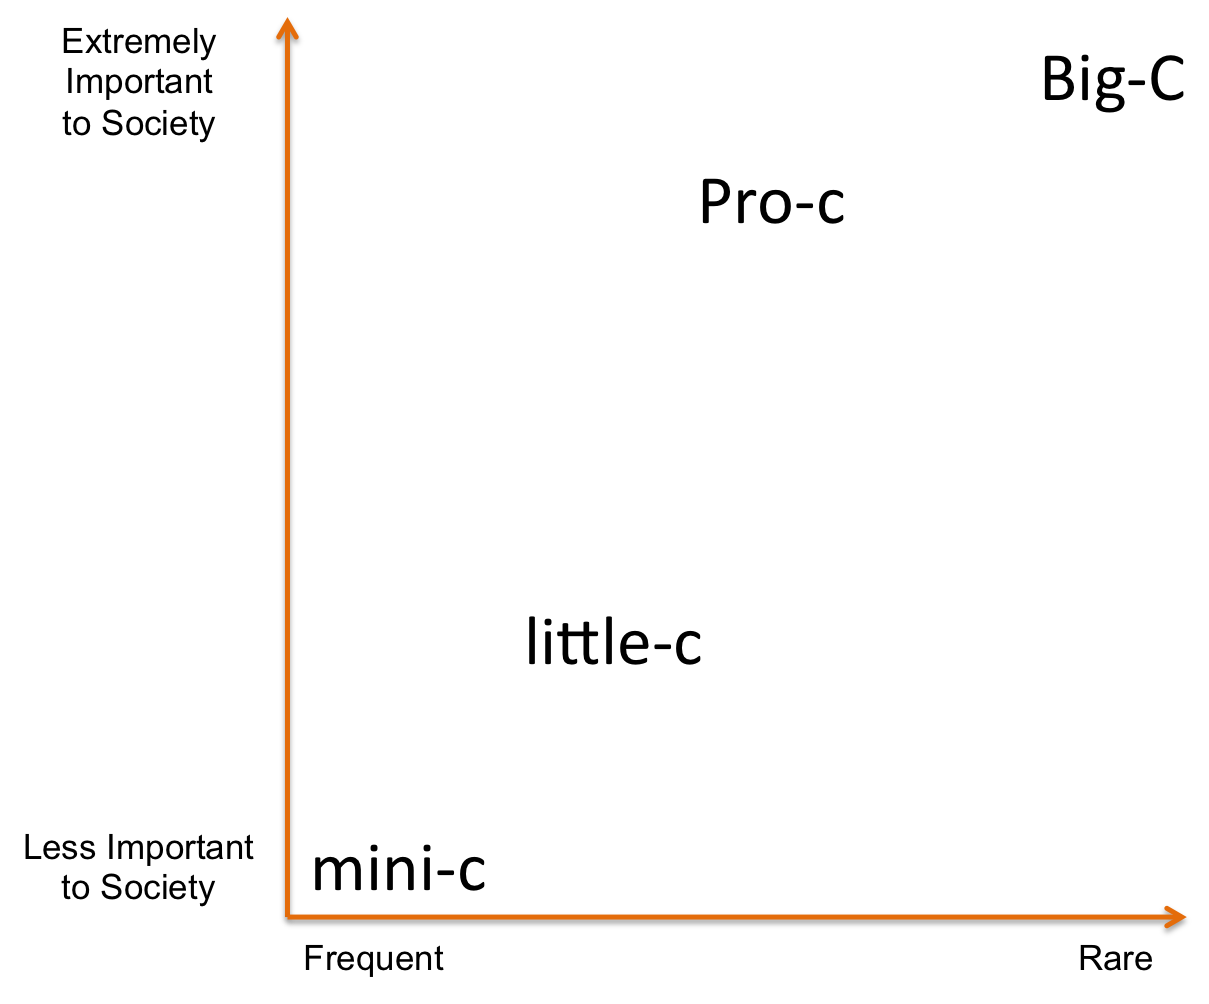
\includegraphics[width=4in]{images/spectrum.png}
\caption{The creativity literature contains classifications of creative contributions across two dimensions: the Novelty-Impact space. Highly novel contributions are more rare, contributions with minimal novelty are more frequent.}
\end{figure}

\bodysection{I have a super super super super super super super super super super super long title}
\bodysubsection{Another super super super super super super super super super super super super super super long title}

\bodysubsection{Evaluation of Creativity Support Tools}
\label{CSTEvaluation}
While there is an extensive history of evaluating creativity, the evaluation of tools to support creativity is a much newer field of study. As previously discussed, Shneiderman noted that the evaluation of creativity support tools is challenging because there are no obvious metrics for researchers to quantify~\cite{Shneiderman:2007wp}. 
